\chapter{\sffamily Interacting with systems in general}

{\bfseries\sffamily Concept.} To design and build a software which can interact with stochastic processes of any kind, either manually through user input, or automatically by introducing a `policy'. The mathematical formalism and software that we introduce here will serve as a common language and interface for any simulation studies into manipulating real world phenomena, and will enable the learning of control algorithms in later chapters of this book. We will implement this new interaction software as an extension to the stochadex package. For the mathematically-inclined, this chapter will cover how interactions are structured in theory by adding some new concepts to the stochadex formalism and illustrating with some simple examples. For the programmers, the public Git repository for the code described in this chapter can be found here: \href{https://github.com/umbralcalc/stochadex}{https://github.com/umbralcalc/stochadex}.

\section{\sffamily Formalising general interactions}

Let's start by considering how we might adapt the mathematical formalism we have been using so far to be able to take actions which can manipulate the state at each timestep. Using the mathematical notation that we inherited from the stochadex, we may extend the formula for updating the state history matrix $X'\rightarrow X$ to include a new layer of possible interactions which is facilitated by a new vector-valued `take action' function $G_{{\sf t}}$. In doing so we shall be defining the domain of an acting entity in the stochastic process environment --- which we shall hereafter refer to as simply the `agent'.

During a timestep over which actions are performed by the agent, the stochadex state update formula can be extended to look to include interactions by composition with the original state update function like so
%%
\begin{align}
X_{{\sf t}+1}^i &= G^i_{{\sf t}+1}[F_{{\sf t}+1}(X', z, {\sf t}), A_{{\sf t}+1}] = {\cal F}^i_{{\sf t}+1}(X', z, A_{{\sf t}+1}, {\sf t}) \label{eq:generalised-state-actions} \,,
\end{align}
%%
where we have also introduced the concept of the `actions' performed $A_{{\sf t}+1}$ on the system; some vector of parameters which define what actions are taken at timestep ${\sf t}+1$.

The code for the new iteration formula given by Eq.~(\ref{eq:generalised-state-actions}), which includes taking actions in the same timestep, would look something like Fig.~\ref{fig:iterations-with-actions}.

\begin{figure}[h]
\centering
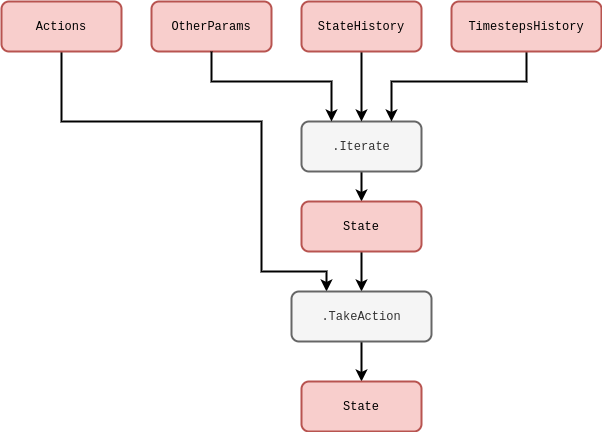
\includegraphics[width=11cm]{images/chapter-9-iterations-with-actions.drawio.png}
\caption{Code schematic of Eq.~(\ref{eq:generalised-state-actions}).}
\label{fig:iterations-with-actions}
\end{figure}

So far, Eq.~(\ref{eq:generalised-state-actions}) on its own will allow the agent to take actions that are scheduled up front through some fixed process or through user interaction via a game interface. So what's next? In order to start creating algorithms which will act on the system state for us, we need to develop a formalism which `closes the loop' by feeding information back from the stochastic process to the agent's decision-making algorithm. Note that in most cases, the state of real-world phenomena cannot be measured perfectly. So to enable any agent trained on simulated phenomena to potentially act in the real world, we will need to include a measurement process as part of the information retrieval step.

When an agent takes an action to measure the state of the system (or when it is given measurements without needing to take action) there will typically be some uncertainty in how the history of measured real-world data $Y$ maps to the latent state of the system $x$ and its parameters $z$ at time ${\sf t}+1$. It is natural, then, to represent this uncertainty with a posterior probability distribution ${\cal P}_{{\sf t}+1}(x,z\vert Y)$ as we did in the previous chapters of this book. 

Let us now define a fully general Non-Markovian Decision Process (NMDP) as a probabilistic model which draws the next action $a=A_{{\sf t}+1}$ from the following distribution
%%
\begin{align}
P_{{\sf t}+1}(a\vert A',\theta) &= \int_{\Omega_{{\sf t}}} {\rm d}X' \, \Pi_{({\sf t}+1){\sf t}}(a\vert X',A',\theta){\cal P}_{{\sf t}}(X'\vert Y') \,.
\end{align}
%%
There's also an updated iteration formula for the stochastic process state which takes the effect of agent actions into account
%%
\begin{align}
P_{{\sf t}+1}(X\vert z,A) &= \int_{\Omega_{{\sf t}'}}{\rm d}X' P_{{\sf t}}(X'\vert z, A') P_{({\sf t}+1){\sf t}}(X\vert X',z,A) \,.
\end{align}
%%


\textcolor{red}{
got to here --- remember to add examples later on
}

If we now define the conditional probability that an action vector element $A_{{\sf t}+1}=a$ is chosen given that the state history up to this point is $X'$ has been measured $\pi (a,x) = p(a\vert x)$, we can use this to draw new actions for the agent with an action-generating function
%%
\begin{align}
A_{{\sf t}+1}^i &= \Pi_{{\sf t}+1}^i(X', z, A', v) \label{eq:action-generating-function} \,.
\end{align}
%%
From this point on we'll call $\pi (a,x)$ the `policy' adoped by the agent. A Markov Decision Process (MDP) defines an algorithm in which the agent uses a single state measurement vector and its given policy $\pi$ to draw actions $A_{{\sf t}+1}$ at timestep ${{\sf t}+1}$. As a reminder; it then takes these actions by interacting with the system using Eq.~(\ref{eq:generalised-state-actions}).

In this equation notice that, in addition to the constant vector of parameters $z$ (as in the stochadex formalism), we have introduced a new time-dependent vector of other parameters $Z_{{\sf t}+1}$ that may be updated by the agent at any (but not necessarily every) timestep. This vector represents the parameters which will be used to define agent behaviour in due course.